\documentclass[twocolumn,10pt]{article}

\usepackage[dvips]{graphicx}
%\usepackage{times}
\usepackage{fullpage}
\usepackage{eprint}
\usepackage{rotating}
\usepackage{eepic}
\usepackage{amsfonts}
\usepackage{algorithmic}
\usepackage{amsthm}

\theoremstyle{plain}
\newtheorem{theorem}{Theorem}

\title{Quantum compiling with Kitaev-Shen-Vyalyi}
\date{December 20, 2011}
\author{Paul Pham}

%    Q-circuit version 1.06
%    Copyright (C) 2004  Steve Flammia & Bryan Eastin

%    This program is free software; you can redistribute it and/or modify
%    it under the terms of the GNU General Public License as published by
%    the Free Software Foundation; either version 2 of the License, or
%    (at your option) any later version.
%
%    This program is distributed in the hope that it will be useful,
%    but WITHOUT ANY WARRANTY; without even the implied warranty of
%    MERCHANTABILITY or FITNESS FOR A PARTICULAR PURPOSE.  See the
%    GNU General Public License for more details.
%
%    You should have received a copy of the GNU General Public License
%    along with this program; if not, write to the Free Software
%    Foundation, Inc., 59 Temple Place, Suite 330, Boston, MA  02111-1307  USA

\usepackage[matrix,frame,arrow]{xy}
\usepackage{amsmath}
\newcommand{\bra}[1]{\left\langle{#1}\right\vert}
\newcommand{\ket}[1]{\left\vert{#1}\right\rangle}
    % Defines Dirac notation.
\newcommand{\qw}[1][-1]{\ar @{-} [0,#1]}
    % Defines a wire that connects horizontally.  By default it connects to the object on the left of the current object.
    % WARNING: Wire commands must appear after the gate in any given entry.
\newcommand{\qwx}[1][-1]{\ar @{-} [#1,0]}
    % Defines a wire that connects vertically.  By default it connects to the object above the current object.
    % WARNING: Wire commands must appear after the gate in any given entry.
\newcommand{\cw}[1][-1]{\ar @{=} [0,#1]}
    % Defines a classical wire that connects horizontally.  By default it connects to the object on the left of the current object.
    % WARNING: Wire commands must appear after the gate in any given entry.
\newcommand{\cwx}[1][-1]{\ar @{=} [#1,0]}
    % Defines a classical wire that connects vertically.  By default it connects to the object above the current object.
    % WARNING: Wire commands must appear after the gate in any given entry.
\newcommand{\gate}[1]{*{\xy *+<.6em>{#1};p\save+LU;+RU **\dir{-}\restore\save+RU;+RD **\dir{-}\restore\save+RD;+LD **\dir{-}\restore\POS+LD;+LU **\dir{-}\endxy} \qw}
    % Boxes the argument, making a gate.
\newcommand{\meter}{\gate{\xy *!<0em,1.1em>h\cir<1.1em>{ur_dr},!U-<0em,.4em>;p+<.5em,.9em> **h\dir{-} \POS <-.6em,.4em> *{},<.6em,-.4em> *{} \endxy}}
    % Inserts a measurement meter.
\newcommand{\measure}[1]{*+[F-:<.9em>]{#1} \qw}
    % Inserts a measurement bubble with user defined text.
\newcommand{\measuretab}[1]{*{\xy *+<.6em>{#1};p\save+LU;+RU **\dir{-}\restore\save+RU;+RD **\dir{-}\restore\save+RD;+LD **\dir{-}\restore\save+LD;+LC-<.5em,0em> **\dir{-} \restore\POS+LU;+LC-<.5em,0em> **\dir{-} \endxy} \qw}
    % Inserts a measurement tab with user defined text.
\newcommand{\measureD}[1]{*{\xy*+=+<.5em>{\vphantom{#1}}*\cir{r_l};p\save*!R{#1} \restore\save+UC;+UC-<.5em,0em>*!R{\hphantom{#1}}+L **\dir{-} \restore\save+DC;+DC-<.5em,0em>*!R{\hphantom{#1}}+L **\dir{-} \restore\POS+UC-<.5em,0em>*!R{\hphantom{#1}}+L;+DC-<.5em,0em>*!R{\hphantom{#1}}+L **\dir{-} \endxy} \qw}
    % Inserts a D-shaped measurement gate with user defined text.
\newcommand{\multimeasure}[2]{*+<1em,.9em>{\hphantom{#2}} \qw \POS[0,0].[#1,0];p !C *{#2},p \drop\frm<.9em>{-}}
    % Draws a multiple qubit measurement bubble starting at the current position and spanning #1 additional gates below.
    % #2 gives the label for the gate.
    % You must use an argument of the same width as #2 in \ghost for the wires to connect properly on the lower lines.
\newcommand{\multimeasureD}[2]{*+<1em,.9em>{\hphantom{#2}}\save[0,0].[#1,0];p\save !C *{#2},p+LU+<0em,0em>;+RU+<-.8em,0em> **\dir{-}\restore\save +LD;+LU **\dir{-}\restore\save +LD;+RD-<.8em,0em> **\dir{-} \restore\save +RD+<0em,.8em>;+RU-<0em,.8em> **\dir{-} \restore \POS !UR*!UR{\cir<.9em>{r_d}};!DR*!DR{\cir<.9em>{d_l}}\restore \qw}
    % Draws a multiple qubit D-shaped measurement gate starting at the current position and spanning #1 additional gates below.
    % #2 gives the label for the gate.
    % You must use an argument of the same width as #2 in \ghost for the wires to connect properly on the lower lines.
\newcommand{\control}{*-=-{\bullet}}
    % Inserts an unconnected control.
\newcommand{\controlo}{*!<0em,.04em>-<.07em,.11em>{\xy *=<.45em>[o][F]{}\endxy}}
    % Inserts a unconnected control-on-0.
\newcommand{\ctrl}[1]{\control \qwx[#1] \qw}
    % Inserts a control and connects it to the object #1 wires below.
\newcommand{\ctrlo}[1]{\controlo \qwx[#1] \qw}
    % Inserts a control-on-0 and connects it to the object #1 wires below.
\newcommand{\targ}{*{\xy{<0em,0em>*{} \ar @{ - } +<.4em,0em> \ar @{ - } -<.4em,0em> \ar @{ - } +<0em,.4em> \ar @{ - } -<0em,.4em>},*+<.8em>\frm{o}\endxy} \qw}
    % Inserts a CNOT target.
\newcommand{\qswap}{*=<0em>{\times} \qw}
    % Inserts half a swap gate. 
    % Must be connected to the other swap with \qwx.
\newcommand{\multigate}[2]{*+<1em,.9em>{\hphantom{#2}} \qw \POS[0,0].[#1,0];p !C *{#2},p \save+LU;+RU **\dir{-}\restore\save+RU;+RD **\dir{-}\restore\save+RD;+LD **\dir{-}\restore\save+LD;+LU **\dir{-}\restore}
    % Draws a multiple qubit gate starting at the current position and spanning #1 additional gates below.
    % #2 gives the label for the gate.
    % You must use an argument of the same width as #2 in \ghost for the wires to connect properly on the lower lines.
\newcommand{\ghost}[1]{*+<1em,.9em>{\hphantom{#1}} \qw}
    % Leaves space for \multigate on wires other than the one on which \multigate appears.  Without this command wires will cross your gate.
    % #1 should match the second argument in the corresponding \multigate. 
\newcommand{\push}[1]{*{#1}}
    % Inserts #1, overriding the default that causes entries to have zero size.  This command takes the place of a gate.
    % Like a gate, it must precede any wire commands.
    % \push is useful for forcing columns apart.
    % NOTE: It might be useful to know that a gate is about 1.3 times the height of its contents.  I.e. \gate{M} is 1.3em tall.
    % WARNING: \push must appear before any wire commands and may not appear in an entry with a gate or label.
\newcommand{\gategroup}[6]{\POS"#1,#2"."#3,#2"."#1,#4"."#3,#4"!C*+<#5>\frm{#6}}
    % Constructs a box or bracket enclosing the square block spanning rows #1-#3 and columns=#2-#4.
    % The block is given a margin #5/2, so #5 should be a valid length.
    % #6 can take the following arguments -- or . or _\} or ^\} or \{ or \} or _) or ^) or ( or ) where the first two options yield dashed and
    % dotted boxes respectively, and the last eight options yield bottom, top, left, and right braces of the curly or normal variety.
    % \gategroup can appear at the end of any gate entry, but it's good form to pick one of the corner gates.
    % BUG: \gategroup uses the four corner gates to determine the size of the bounding box.  Other gates may stick out of that box.  See \prop. 
\newcommand{\rstick}[1]{*!L!<-.5em,0em>=<0em>{#1}}
    % Centers the left side of #1 in the cell.  Intended for lining up wire labels.  Note that non-gates have default size zero.
\newcommand{\lstick}[1]{*!R!<.5em,0em>=<0em>{#1}}
    % Centers the right side of #1 in the cell.  Intended for lining up wire labels.  Note that non-gates have default size zero.
\newcommand{\ustick}[1]{*!D!<0em,-.5em>=<0em>{#1}}
    % Centers the bottom of #1 in the cell.  Intended for lining up wire labels.  Note that non-gates have default size zero.
\newcommand{\dstick}[1]{*!U!<0em,.5em>=<0em>{#1}}
    % Centers the top of #1 in the cell.  Intended for lining up wire labels.  Note that non-gates have default size zero.
\newcommand{\Qcircuit}{\xymatrix @*=<0em>}
    % Defines \Qcircuit as an \xymatrix with entries of default size 0em.


\begin{document}

%\newcommand{\ket}[1]{|#1 \rangle}
%\newcommand{\bra}[1]{\langle #1 |}
\newcommand{\braket}[2]{\langle #1|#2 \rangle}
\newcommand{\normtwo}{\frac{1}{\sqrt{2}}}
\newcommand{\norm}[1]{\parallel #1 \parallel}

\maketitle

\section{Abstract}

Quantum compilers approximate high-level circuits for quantum algorithms
into a universal, machine-dependent
instruction set that can be implemented by experiment. This work contributes
a numerical comparison of the
resources needed to run two quantum compiling procedures on single-qubit gates,
along with the underlying open source code.
The first is the well-known Solovay-Kitaev procedure, which uses no ancillae and
is completely classical. The second is the lesser-known result by Kitaev,
Shen, and Vyalyi which reduces compiled
circuit depth using parallelization at the expense of more ancilla qubits and
a quantum component that must be executed at runtime.
We also provide a pedagogical review of this second procedure as an aid to
future implementation and comment on some considerations of future
quantum architectures regarding compilation.

\section{Introduction}

Quantum computers can achieve exponential speedups over known classical
algorithms in theory. For example, Shor's factoring algorithm can break the
widely-used RSA cryptosystem, and quantum many-body systems can only be
efficiently simulated by quantum algorithms [paper citations needed].
However, this speedup can be mitigated or lost completely when implementing
these algorithms in a physical experiment.
Two important implementation considerations 
are fault-tolerance and architecture. We do not address the vast topic
of fault-tolerance (including error correction) here, and instead
concentrate on compiling, which we include in the domain of architecture.

\emph{Quantum compiling} is the
approximation of a high-level quantum algorithm (usually described as a
reversible circuit) using a sequence
of low-level, universal quantum gates that depend on our hardware, the
"assembly language" of quantum computing.
At the highest-level of abstraction, all quantum algorithms on $n$ qubits
can be considered as a unitary matrix of dimension $2^n \times 2^n$ with
unit determinant, followed by measurement (and perhaps several rounds of this).
However, in experimental settings,
we can only perform some gates efficiently, and these are usually local
(nearest-neighbor) two-qubit or single-qubit operations.
Moreover, most of our results for fault-tolerant
quantum computing in the presence of noise stipulates that we have a finite
number of universal gates we can perform with some limited precision.

Several quantum compiling procedures are currently known. The first one,
by Solovay and Kitaev (SK),
is a central results of quantum computing which states that we
can approximate quantum gates efficiently in circuit size and
depth (i.e. without losing any exponential speedup) \cite{Dawson2005}.
A second procedure due to Kitaev, Shen, and Vyalyi (KSV) is more recent but
less well-known, improves
both the depth and size of the SK procedure by trading
more ancillae (space) for time (depth) using parallelism
\cite{ksv02}. Several other quantum compiling approaches are described
in the next section. However, the KSV procedure is unique in its combination of
various theoretical tools and warrants a dedicated comparison.

This work contributes the calculation of physical resources needed
to run the SK and KSV quantum compilers on a single-qubit phase gate
of the form $\ket{0}\bra{0} + e^{i\phi}\ket{1}\bra{1}$, for reasons that
will soon become clear. We also contribute open source code to duplicate
these results, which is available at \texttt{http://quantum-compiler.org}.
Finally, we give a pedagogical review of KSV and its building blocks from the
perspective of implementation on an architecture allowing arbitrary concurrent
operations. This model is known as \textsc{AC} in the literature.
\cite{VanMeter2008}. Therefore, this current work can be read in combination
with Chapter 13 of \cite{ksv02} to gain a full understanding of the KSV
compiler.

The rest of this report is organized as follows.
First, Section \ref{sec:prelims} defines terms and parameters
so that we can discuss quantum compilers with some rigor as well as
giving asymptotic bounds for specific algorithms.
Then Section
\ref{sec:related} gives a brief history of quantum compiling.
The next two sections describe the two compiling algorithms and how
to measure their relative performance.
Section \ref{sec:sk-algo} reviews the original SK result and
Section \ref{sec:main-algo} describes the building blocks of KSV in detail
along with its
most resource-intensive modules. Section \ref{sec:methods} describe
our methods for the performance comparisons, which are given in Section
\ref{sec:results}. Finally, we make some comments about these results
and suggest future directions for extending this work.

\section{Preliminaries}
\label{sec:prelims}

%%%%%%%%%%%%%%%%%%%%%%%%%%%%%%%%%%%%%%%%%%%%%%%%%%%%%%%%%%%%%%%%%%%%%%%%%%%%%%
\subsection{Some Special Operator Notation}

Borrowing the notation in \cite{ksv02},
we define two controlled ``meta-operators'' which takes some unitary $U$ as
a parameter. The first describes a controlled-$U$ operation where the control
is a single qubit.

\begin{displaymath}
\Lambda(U) = \ket{0}\bra{0} \otimes I + \ket{1}\bra{1} \otimes U
\end{displaymath}

The second describes a registered-$U$ operation, which
can be thought of as applying $U^p$ to some target register
controlled on a separate $m$-qubit register
encoding the number $p$.

\begin{displaymath}
\Upsilon_m(U) : \ket{p} \otimes \ket{\psi} \rightarrow \ket{p}
\otimes U^p\ket{\psi}
\end{displaymath}

Note that $\Upsilon_1(U)$ and $\Lambda(U)$ are equivalent.

%%%%%%%%%%%%%%%%%%%%%%%%%%%%%%%%%%%%%%%%%%%%%%%%%%%%%%%%%%%%%%%%%%%%%%%%%%%%%%
\subsection{A Universal Set of Gates}

We use the following universal standard set of gates $\mathcal{G}$ throughout
this paper.

\begin{displaymath}
\mathcal{G} = \{ H, K, K^{\dagger}, X, Z,
\Lambda(\sigma_x), \Lambda^2(\sigma_x) \}
\end{displaymath}

These gates all operate on single qubits with the
exception of $\Lambda(\sigma_x)$ (the two-qubit CNOT gate)
and $\Lambda^2(\sigma_x)$ (the three-qubit Toffoli gate),
which can be interpreted as singly- and doubly-controlled
$X$ gates, respectively. $X$ and $Z$ are the standard Pauli matrices
$\sigma_x$ and $\sigma_z$, $H$ is the Hadamard matrix, and $K$ and its
Hermitian conjugate $K^{\dagger}$ are phase gates of $i$ and $-i$,
respectively.

\begin{displaymath}
Z = 
 \left[
  \begin{array}{cc}
    1 & 0 \\
    0 & -1 \\
  \end{array} \right]
\qquad
X = 
 \left[
  \begin{array}{cc}
    0 & 1 \\
    1 & 0 \\
  \end{array} \right]
\end{displaymath}

\begin{displaymath}
K = 
 \left[
  \begin{array}{cc}
    1 & 0 \\
    0 & i \\
  \end{array} \right]
\qquad
K^{\dagger} = 
 \left[
  \begin{array}{cc}
    1 & 0 \\
    0 & -i \\
  \end{array} \right]
\end{displaymath}

Without proving the universality of $\mathcal{G}$, we note that there are
methods for expressing any $2^n \times 2^n$ unitary matrix as a
tensor product of single- and two-qubit gates \cite{Bremner2002}. We call
the process of decomposing elements of $SU(N)$ into elements of
$SU(2)$ and $SU(4)$ \emph{quantum circuit synthesis}
[citation to Markov]
to distinguish them as
an intermediate stage in quantum compiling, for which procedures like SK and
KSV provide the final stage of producing circuits formed from $\mathcal{G}$.

%%%%%%%%%%%%%%%%%%%%%%%%%%%%%%%%%%%%%%%%%%%%%%%%%%%%%%%%%%%%%%%%%%%%%%%%%%%%%%
\subsection{Parameters}

The problem of quantum compiling is to translate
an entire circuit $C$ of $S$ gates with depth
$D$ to a new, compiled circuit $C'$ of size $S'$ and depth $D'$ which approximates
$C$ within error $\epsilon$ using some distance measure.

%%%%%%%%%%%%%%%%%%%%%%%%%%%%%%%%%%%%%%%%%%%%%%%%%%%%%%%%%%%%%%%%%%%%%%%%%%%%%%
%%%%%%%%%%%%%%%%%%%%%%%%%%%%%%%%%%%%%%%%%%%%%%%%%%%%%%%%%%%%%%%%%%%%%%%%%%%%%%
% Figure out what you are actually measuring / calculating in your code
$S$ is measured in the number of gates from $\mathcal{G}$. $D$ is measured in
number of concurrent timesteps of ... $W$ is measured in total number of 
ancillae qubits needed to maintain a coherent state for the duration of the
computation.

In our code, we use the trace measure introduced by Austin Fowler which disregards
the global phase factor. Here,
$d$ refers to the dimensionality
of our system ($d = 2^n$ for $n$ qubits).

\begin{equation}
d(U,\tilde{U}) = \sqrt{\frac{d - \norm{\mathrm{tr}(U^\dagger \tilde{U})}}{d}}
\end{equation}

We will use the terms ``error'', ``precision'', and
``accuracy'' interchangeably when approximating gates.
There is some overhead in the compiled circuit, so in
general $C'$ is larger (that is, $S' > S$ and $D' > D$). It's also known that
in order to approximate a circuit with $S$ gates to a total precision of
$\epsilon$
requires each gate to be approximated to a precision of
$n = O(\log(S/\epsilon)$ \cite{Lloyd1995}. We denote this per-gate precision
$n$, since it serves as an independent parameter for compiling. We will clarify
where there is confusion with using $n$ to denote the number of qubits in a
register or being acted upon by a circuit.
We denote at $T$ the classical preprocessing time to
produce $C'$.
 
Circuit depth is analogous to running time, or how long we have to wait from
feeding in inputs to getting a correct output. Relative to the circuit size,
it is a heuristic for how parallelizable our
circuit is. For example, in a single ion trap, if we had multiple lasers,
we could ``flatten'' our circuit into layers with bounded fan-in and
fan-out and operate on multiple ions in parallel.
We could also operate multiple ion traps in parallel which communicate by
teleportation.
All other things being equal, a circuit with low depth will complete
faster than one with high depth, although in practice we can only execute
fixed-width circuits.

%%%%%%%%%%%%%%%%%%%%%%%%%%%%%%%%%%%%%%%%%%%%%%%%%%%%%%%%%%%%%%%%%%%%%%%%%%%%%%
\subsection{Quantum Coprocessor Model}

All experimental implementations of quantum computers treat them as an
auxiliary device controlled by a classical computer. This is the way
quantum computers will function for the foreseeable future, and many
quantum algorithms can be split into classical and quantum parts
to reflect this distinction. The existence of classical control in this
``quantum coprocessor'' model is useful not only in quantum compiling but
also allows us to perform certain quantum circuits in constant depth
[citation needed for fanout and parity].

For example,
SK is a completely classical procedure which is run before
the quantum algorithm to yield a deterministic set of gates. KSV
also contains classical side-processing as part of its parallelized
phase-estimation. We will neglect the performance of these classical parts
since they are polynomial in time or space, with one exception. We will
discuss the classical space overhead of SK in Section \ref{subsec:results-width}.

On a related note, we may choose to projectively measure some ancilla qubits
in the middle of a quantum algorithm in order to offload some (polynomial-time)
processing to the classical controller.
These ancillae then contain garbage values and
cannot be used for the remainder of the computation. From a practical point of
view, this ``one-shot'' method is worth doing if the number of such
wasted qubits is small compared to the reduction in the quantum circuit size.
We discuss our use of this technique in Section \ref{subsec:ppe} for parallelized
phase estimation.

The alternative is sometimes
called ``coherent measurements'' or ``simulating measurements'' \cite{Cleve2000}
in which some operation is controlled on the quantum value to be measured and
can be reversed later to recover ancillae at the cost of a larger quantum circuit.

%%%%%%%%%%%%%%%%%%%%%%%%%%%%%%%%%%%%%%%%%%%%%%%%%%%%%%%%%%%%%%%%%%%%%%%%%%%%%%
\subsection{Asymptotic Circuit Bounds}

The SK and KSV algorithms compile circuits with
a size and depth which depend on the desired per-gate precision $n$.
These asymptotic bounds are listed in
Table \ref{tab:asymptotics}, which actually refer to an improved version of
SK described in Theorem 8.5 of \cite{ksv02}, where 
$\nu$ is a small positive constant.
However, we describe a simpler version of SK in Section \ref{sec:sk-algo}
which has a fixed exponent of about $c=3.97$, which is easier to understand,
and does not significantly change the asymptotic relationship between SK and
KSV.

We will see these asymptotic bounds reflected
later in the actual numerical results in Section \ref{sec:results}.

\begin{center}
\begin{table}
\label{tab:asymptotics}
\begin{tabular}{|c|c|c|}
\hline
   & SK & KSV \\
\hline
$S'$ & $O(Sn^{3+\nu})$ & $O(Sn + n^2 \log n)$\\
$D'$ & $O(Dn^{3+\nu})$ & $O(D \log{n} + (\log{n})^2))$\\ 
$W'$ & $0$             & $$ \\
\hline
\end{tabular}
\caption{Asymptotic circuit resources for SK and KSV compilers}
\end{table}
\end{center}

\section{Related Work}
\label{sec:related}

In 1995, Seth Lloyd found that almost any two distinct single-qubit rotations are
universal for approximating an arbitrary single-qubit rotation, but that this
approximation could be exponentially long in the desired per-gate error $n$
for both time and length, that is,
$T,L = O(1/\epsilon)$ for $\epsilon = O(2^{-n})$ \cite{Lloyd1995}.

The theorem which is now called Solovay-Kitaev was discovered by Solovay in
1995 in an unpublished manuscript and independently later discovered by
Kitaev in 1997 \cite{nc00} which showed that $T,L = O(\log^c{1/\epsilon})$ for
$c$ between 3 and 4, showing for the first time that quantum compiling
could be efficient.

In 2001, Aram Harrow completed his undergrad thesis arguing that it would be difficult
to beat $c < 2$ for the above bounds using a successive approximation
method \cite{harrow01}.

In 2002, Kitaev, Shen, and Vyalyi published their book which contains an
application of parallelized phase estimation towards simulating a quantum
circuit (what we are calling KSV) \cite{ksv02}.
That is, KSV is an alternative quantum compiler to SK which has
asymptotically better circuit depth and circuit size, constant classical
preprocessing time ($T=O(1)$),
but using ancillary qubits (increased circuit width).

In 2003, Harrow, Recht, and Chuang demonstrated that a certain universal
set could be used to saturate the lower bound $L=O(\log{1/\epsilon})$
but it remains an open problem whether any efficient algorithm exists
which can do this in tractable $T$ \cite{hrc02}.

In 2005, Dawson and Nielsen published their pedagogical review
paper of Solovay-Kitaev \cite{Dawson2005}.

In 2010, Burrello, Mussardo, and Wan discovered a quantum compiler for
topological quantum computing which saturates the lower bound ($c=1$) for
non-Abelian anyons \cite{Burrello2010}.

%%%%%%%%%%%%%%%%%%%%%%%%%%%%%%%%%%%%%%%%%%%%%%%%%%%%%%%%%%%%%%%%%%%%%%%%%%%%%%
%%%%%%%%%%%%%%%%%%%%%%%%%%%%%%%%%%%%%%%%%%%%%%%%%%%%%%%%%%%%%%%%%%%%%%%%%%%%%%
% Write up references to Tucci and Markov and circuit synthesis papers
% put in the right chronological order as above

\section{Review of Solovay-Kitaev}
\label{sec:sk-algo}

The essential structure of SK is to recursively generate nets of unitary
operators with
successively finer precision. At any given level of recursion, the input 
gate is divided up into two halves which are further from identity [is this
really true] and can be
approximated with less precision. Our pseudo-code and explanation
follows the exposition in \cite{Dawson2005} and \cite{harrow01}

\begin{algorithmic}[1]
\STATE \textsc{function} $\tilde{U}_i \leftarrow$ SK$(U,n)$
\IF{$i == 0$}
\STATE $\tilde{U}_i \leftarrow $ BASIC-APPROX$(U)$
\ELSE
\STATE $\tilde{U}_{i-1} \leftarrow$ SK$(U, i-1)$
\STATE $A,B \leftarrow $ FACTOR$(U\tilde{U}^\dagger_{i-1})$
\STATE $\tilde{A}_{i-1} \leftarrow $ SK$(A, i-1)$
\STATE $\tilde{B}_{i-1} \leftarrow $ SK$(B, i-1)$
\STATE $\tilde{U}_i \leftarrow \tilde{A}_{i-1}\tilde{B}_{i-1}\tilde{A}^\dagger_{i-1}\tilde{B}^\dagger_{i-1}\tilde{U}_{i-1}$
\ENDIF
\STATE return $\tilde{U}_i$
\end{algorithmic}

Since the recursion must eventually bottom out, we must precompute some sequences
of gates from $\mathcal{G}$ up to length $l_0$. This is the classical
preprocessing step which requires upfront storage space for this
coarsest-grained net, where
each sequence is no more than $\epsilon_0$ from its nearest neighbor. According
to \cite{Dawson2005} the values of $l_0=16$ and $\epsilon_0 = 0.14$ using
operator norm distance is sufficient for most applications.
This step can be
done offline and reused across multiple runs of the compiler, assuming
$\mathcal{G}$ for your quantum computer doesn't change.

The BASIC-APPROX function above does a lookup (e.g. using some kd-tree search
maneuvers through higher-dimensional vector spaces) using this $\epsilon_0$-net,
and all higher recursive calls to SK are effectively constructing
finer $\epsilon$-nets on the fly as needed.

The FACTOR function performs a balanced group commutator decomposition,
$U = ABA^\dagger B^\dagger$, and then recursively approximates the $A$ and $B$
operators, again using SK. We denote by $\tilde{U}_i$ as the approximation
of $U$ using $i$ levels of SK recursion. Intuitively, when they are multiplied
together again, along with their inverses, their errors (which go like
$\epsilon$) are symmetric and cancel out in such a way that the resulting
product $U$ has errors which go like $\epsilon^2$. In this manner, we can
eventually sharpen our desired error down to any value. We use the
geometric decomposition in \cite{Dawson2005} rather than the decomposition
based on a BCH-like approximation as in \cite{harrow01}, although it is not
known which method converges more quickly to a desired gate in general.

%%%%%%%%%%%%%%%%%%%%%%%%%%%%%%%%%%%%%%%%%%%%%%%%%%%%%%%%%%%%%%%%%%%%%%%%%%%%%%%
%%%%%%%%%%%%%%%%%%%%%%%%%%%%%%%%%%%%%%%%%%%%%%%%%%%%%%%%%%%%%%%%%%%%%%%%%%%%%%%
% we still need to reconcile this 5^n with log^{3.97}(1/\epsilon)
% this is an evernote item, maybe it is already reconciled

Each level $i$ of recursion solves the problem of compiling 
$U_i$ by combining five gates compiled at the lower $i-1$ level.
Therefore, the compiled circuit size at the top-level is upper-bounded by $5^n$,
and
this is in general the same as the circuit depth (since not all gates in
$\mathcal{G}$ commute).

%%%%%%%%%%%%%%%%%%%%%%%%%%%%%%%%%%%%%%%%%%%%%%%%%%%%%%%%%%%%%%%%%%%%%%%%%%%%%%%
%%%%%%%%%%%%%%%%%%%%%%%%%%%%%%%%%%%%%%%%%%%%%%%%%%%%%%%%%%%%%%%%%%%%%%%%%%%%%%%
% we still need a discussion somewhere of the relationship between commuting
% operators and parallelizing them into the same timestep

\section{The KSV Procedure}
\label{sec:main-algo}

KSV takes a radically different approach than SK by identifying that most gates
can be easily constructed from sequences in
$\mathcal{G}$ in constant time with the exception of the ``targetless''
controlled phase operator, which takes the most work to approximate.

\begin{displaymath}
\Lambda(e^{i\phi}) = 
 \left(
  \begin{array}{cc}
    1 & 0 \\
    0 & e^{i\phi} \\
  \end{array} \right)
\end{displaymath}

\cite{ksv02} is a self-contained reference
for enacting $\Lambda(e^{i\phi})$ with several modules which are useful in
their own right:
parallelized phase estimation, parallel iteration of finite
automata, and a logarithmic depth quantum arithmetic operations such
as addition (and subtraction) described in \ref{subsec:add},
multiplication described in \ref{subsec:mult}, and division described
in \ref{subsec:div}.

In order to do all of this, however, we will need to introduce the eigenstates
of the $\bmod 2^n$ addition operator.

%It is now useful to discuss certain states with remarkable properties.
%Their superposition is easy to form, and they are the eigenstates of a
%$\bmod 2^n$ addition operator which is efficient to implement.
%Used with phase estimation,
%this would allow us to enact
%a particular phase shift, and also to copy these eigenstates,
%simply by adding numbers.

%%%%%%%%%%%%%%%%%%%%%%%%%%%%%%%%%%%%%%%%%%%%%%%%%%%%%%%%%%%%%%%%%%%%%%%%%%%%%%%
\subsection{Addition Eigenstates}
\label{subsec:magic-state}

Suppose you were given the state $\ket{\psi_{n,k}}$
parameterized by the
integers $n$ and $k$ such that

\begin{equation}
\ket{\psi_{n,k}} = \frac{1}{\sqrt{2^n}} \sum_{j=0}^{2^n-1}
e^{-2\pi i j k / 2^n} \ket{j}
\end{equation}

where $0 < k < 2^n$ and $k$ is odd.

Note that these states $\ket{\psi}$ are the
QFT states of the computational basis.
%%%%%%%%%%%%%%%%%%%%%%%%%%%%%%%%%%%%%%%%%%%%%%%%%%%%%%%%%%%%%%%%%%%%%%%%%%%%%%%
%%%%%%%%%%%%%%%%%%%%%%%%%%%%%%%%%%%%%%%%%%%%%%%%%%%%%%%%%%%%%%%%%%%%%%%%%%%%%%%
% actually there is a more precise description here. QFT over 2^n ?
This implicitly argues that these states are hard to create,
because QFT in general requires
$O(n^2)$-depth and we need a logarithmic-depth compiler.
%%%%%%%%%%%%%%%%%%%%%%%%%%%%%%%%%%%%%%%%%%%%%%%%%%%%%%%%%%%%%%%%%%%%%%%%%%%%%%%
%%%%%%%%%%%%%%%%%%%%%%%%%%%%%%%%%%%%%%%%%%%%%%%%%%%%%%%%%%%%%%%%%%%%%%%%%%%%%%%
% we should mention the difficulty even of approximate QFT
% and use circuit size, not depth since constant-depth QFT was shown in
% Brown, Kasheffi, Perdrix (cite here too, just to show off)

However, what we can do is create a superposition over all odd $k=(2s-1)$
by starting in the state $\ket{0}^{\otimes n}$,
then applying a Hadamard and $\sigma^z$ to the most significant qubit.

\begin{equation}
\ket{\eta} = \normtwo \ket{0} - \normtwo \ket{2^{n-1}} =
\frac{1}{\sqrt{2^{n-1}}} \sum_{s=1}^{2^{n-1}} \ket{\psi_{n,2s-1}}
\end{equation}

More obviously relevant to our overall goal of approximating
$\Lambda(e^{i\phi})$, we can enact a phase
shift simply by performing the following modular addition operator, for
which $\ket{\psi_{n,k}}$ are eigenstates.

\begin{equation}
A\ket{j} \rightarrow \ket{j+1 \bmod 2^n}
\end{equation}

Applying this operator to its eigenstates results in a phase shift which
depends on the particular eigenstate.
 
\begin{equation}
A\ket{\psi_{n,k}} = e^{2\pi i \phi_k} \ket{\psi_{n,k}}
\end{equation}

Finding the eigenvalue $e^{2\pi i \phi_k}$ corresponds to finding
the phase $\phi_k = k / 2^n$.
Repeated application of $A$ (say $p$ times) would result in a phase
added to the eigenstate equal to a multiple of $e^{2\pi i p / 2^n}$

\begin{equation}
A^p\ket{\psi_{n,k}} = e^{2\pi i \phi_k / 2^n} \ket{\psi_{n,k}}
\end{equation}

This explains why we don't find even $k$ interesting,
since then we would not get a
cyclic distribution of $2^n$ different phases,
since only odd $k$
are coprime with $2^n$. The exception is $k=0$, since this is the
equal superposition of computational basis states, which we can also
efficiently create. This will be a useful starting point later on to
create addition eigenstates
for odd $k$.

\begin{displaymath}
\ket{\psi_{n,0}} = H^{\otimes n}\ket{0^n}
\end{displaymath}

Suppose we have a certain state $\ket{\psi_{n,k}}$ but we want to get enact
a phase shift $e^{2\pi i l / 2^n}$. We can do this by solving $p=p(s,l)$
in this equation:

\begin{equation}
\label{eqn:psl}
(2s-1)p \equiv l (\bmod 2^n)
\end{equation}

Stipulating $k$ to be odd guarantees that there is a unique solution $p$.

We then apply $A^p$ as follows:

\begin{equation}
\label{eqn:upsilon}
\Upsilon_n(A) \ket{p, \psi_{n,k}} \rightarrow
e^{2\pi i l/2^n} \ket{p, \psi_{n,k}}
\end{equation}

But $p$ is in general hard to solve for, unless $k=1$, in which case
$p = l$. Therefore, we will later see that $\ket{\psi_{n,1}}$ is a desirable
state to have.

Finally, to copy the state $\ket{\psi_{n,k}}$ it suffices to apply the following
operator which only uses subtraction (addition with one addend and the
outcome negated in two's complement representation).

\begin{equation*}
\ket{\psi_{n,k}}^{\otimes m} = W^{-1}\left( \ket{\psi_{n,0}}^\otimes(m-1) \otimes \ket{\psi_{n,k}} \right)
\end{equation*}

where $W$ is the operator on $m$ registers, each of consisting of $n$ qubits,
which adds all the registers into its final register (modulo $2^n$).

\begin{multline}
W : \ket{x_1,\ldots,x_{m-1},x_m} \rightarrow \\
 \ket{x_1,\ldots,x_{m-1},x_1+\ldots+x_m \bmod 2^n}
\end{multline}

Armed with these properties, we're now ready to outline the main steps in KSV.

%For the steps below, we note that we can avoid solving the equation $kp \equiv l (mod 2^n)$
%if we set $k=1$. This is equivalent to realizing $\Upsilon_n(e^{2\pi i / 2^n})$
%by applying $\Upsilon(A)$ from Section \ref{subsec:phase-shift} to the state
%$\ket{\psi_{n,1}}$. So we need to create one copy of this magic state to
%simulate each of $m$ $\Lambda(e^{i\phi})$ gates, $m \le L'$.

%%%%%%%%%%%%%%%%%%%%%%%%%%%%%%%%%%%%%%%%%%%%%%%%%%%%%%%%%%%%%%%%%%%%%%%%%%%%%%%
\subsection{KSV Steps}

Given a circuit $C$ to compile,

\begin{enumerate}
\item Precompile $C$ into gates from $\mathcal{G} \cup \{\Lambda(e^{2\pi i l / 2^n})\}$
using the results from Section \ref{subsec:precompile} in $O(1)$ time, depth,
and size.
Now we are done with the single-qubit gates and CNOT, and we have computed
the values $\{l_1, \ldots , l_m\}$ that allow us to approximate our
desired $m$
$\Lambda(e^{i\phi})$ gates as $\phi \approx l/2^n$ to within precision
$2^{-n}$.
\item Create the state magic state $\ket{\psi_{n,0}}$ with $n$ Hadamards.
\item Turn it into $\ket{\psi_{n,1}} = \Upsilon(e^{-2\pi i / 2^n}) \ket{\psi_{n,0}}$
using the registered phase shift procedure in Section \ref{subsec:phase-shift}
This is done with a circuit of size $O(n^2\log n)$ and $O((\log n)^2)$ depth.
\item Make $m$ copies of the state $\ket{\psi_{n,1}}$ out of one copy by 
applying the addition operation $A$.
\item Simulate each $\Lambda(e^{2\pi i l / 2^n})$
using one copy each of $\ket{\psi_{n,1}}$, to which we can add our
values $l$ using $\Upsilon(A)$.
This takes size $O(mn)$ and depth $O(\log n)$, since we can enact
all these phase shifts in parallel.
\end{enumerate}

Now for the resource calculations of these individual steps and their
substeps.

\subsection{Precompiling to the Standard Set}
\label{subsec:precompile}

This is the completely classical preprocessing step for Super-Kitaev which
assumes we can express any $n$-qubit gate as a tensor product of
single- and two-qubit gates.
From there, how do we get down to our universal set?

%\begin{theorem}[Lemma 8.2]
%\label{lemma82}
%Any arbitrary unitary operator $U$ of dimension $d \times d$ can be represented
%as a product of $d(d-2)/2$ matrices of the form:
%
%\begin{equation*}
%\left( \begin{array}{cccccccc}
%     1 & 0      & \cdots & \cdots & \cdots & \cdots & \cdots & \cdots\\
%     0 & 1      & \cdots & \cdots & \cdots & \cdots & \cdots & \cdots\\
%\vdots & \cdots & \ddots & \cdots & \cdots & \cdots & \cdots & \cdots\\
%\vdots & \cdots & \cdots &      a &      b & \cdots & \cdots & \cdots\\
%\vdots & \cdots & \cdots &      c &      d & \cdots & \cdots & \cdots\\
%\vdots & \cdots & \cdots & \cdots & \cdots & \vdots & \cdots & \cdots\\
%\vdots & \cdots & \cdots & \cdots & \cdots & \cdots & 1 & 0\\
%\vdots & \cdots & \cdots & \cdots & \cdots & \cdots & 0 & 1\\
%\end{array}
%\right)
%\end{equation*}
%
%where $\left( \begin{array}{cc}
%a & b\\
%c & d\\
%\end{array} \right) \in SU(2)$
%\end{theorem}
%
%\begin{proof}
%The running time of this algorithm is $O(M^3) \cdot \mathrm{poly}(\log(1/\delta)$.
%\end{proof}

We use the Euler angle decomposition into $X$ and $Z$ rotations,
we can express any
unitary $U$ as follows, with real angles $\phi$, $\gamma$, $\beta$, $\alpha$:

\begin{equation*}
U = e^{i\phi}e^{i(\gamma/2)\sigma^z}e^{i(\beta/2)\sigma^x}e^{i(\alpha/2)\sigma^z}
\end{equation*}
This involves solving four equations in four variables and can be done in
constant time.

Now how do we implement each of the elements of the Euler angle decomposition from
the $\mathcal{Q}$? Using these identities:

\begin{equation*}
e^{i\phi} = \Lambda(e^{i\phi})\sigma^x\Lambda(e^{i\phi})\sigma^x
\end{equation*}
\begin{equation*}
\sigma^x = H\Lambda(e^{i\pi})H
\end{equation*}
\begin{equation*}
e^{i\phi\sigma^z} = \Lambda(e^{-i\phi}\sigma^x\Lambda(e^{i\phi})\sigma^x
\end{equation*}
\begin{equation*}
e^{i\phi\sigma^x} = H e^{i\phi\sigma^z} H
\end{equation*}

In addition,
any controlled operator $\Lambda(U)$ where $U \in SU(2)$ can be simulated
using
$\mathcal{Q} \cup \{ \Lambda(e^{i\phi})$.

We can represent the controlled operator as $\Lambda(U) = \Lambda(e^{i\phi})\Lambda(V)$.
$\Lambda(e^{i\phi})$ is already in our set, so it remains to implement
$\Lambda(V)$, where $V \in SU(2)$. Geometrically, we can decompose any
three-dimensional rotation into two $180^{\circ}$ rotations about appropriate
axes. Using the homomorphism between $SO(3)$ and $SU(2)$ and the fact that
$\sigma^x$ corresponds to a $180^{\circ}$ rotation about the $x$-axis.

\begin{equation*}
V = A\sigma^x A^{-1} B\sigma^x B^{-1}
\end{equation*}


\subsection{Registered-Phase Shift}
\label{subsec:phase-shift}

Registered phase shifting is the only use of phase estimation in
Super-Kitaev but it is the most resource-intensive step.
We would like to enact the operator $\Upsilon(e^{-2\pi i / 2^n})$ on
$\ket{\psi_{n,0}}$, which is easy to create, to get $\ket{\psi_{n,1}}$,
which we can later use to enact $\Lambda(e^{2\pi i l / 2^n})$.

\begin{enumerate}
\item Create the state $\ket{\eta}$ as described in \ref{subsec:magic-state}.
\item Measure $k$ by determining the phase $\phi_k = k/2^n$ with precision
$\delta = 2^{-n}$ by using phase estimation. One of the $n$-qubit registers
now contains $\ket{\psi_{n,k}}$ for some fixed $k$.
This is done by parallelized phase estimation described in
\ref{subsec:ppe}.
This is done by a circuit of size $O(n^2)$ and depth $O(\log n)$.
\item Solve for $p$ in equation
Equation \ref{eqn:psl} using modular division, described in
\ref{subsec:div}.
\item Apply $A^p$ to the $n$-qubit register containing $\ket{\psi}$, which
enacts the desired phase shift.
\end{enumerate}


\subsection{Parallelized Phase Estimation}
\label{subsec:ppe}

One of the key components of the registered phase shifting procedure
described in the previous section is the ability to ``pick'' a random
eigenstate $\ket{\psi_k}$ of a unitary operator $U$ and
measure its corresponding eigenvalue (phase) $\phi_k$
with some degree of precision $\delta = 2^{-n}$ and
error probability $\epsilon = 2^{-l}$. As $n$ increases, the phases
generally become closer together, which is why we need exponential precision
to distinguish between them.
Of course, this exactly describes the phase
estimation procedure, a key technique in many quantum algorithms developed
by Kitaev in his derivation of Shor's factoring result \cite{kitaev}.

\begin{displaymath}
U\ket{\psi_k} = e^{2\pi i \phi_k} \ket{\psi_k}
\end{displaymath}

Phase estimation holds some superposition of eigenstates
$\sum_{i} \alpha_i \ket{\psi_i}$
in an $n$-qubit target register, to which it applies repeated measuring
operators $\Lambda(U^{2^k})$
controlled on some $t$-qubit register, which holds an
approximation $\tilde{phi}$ to the real phase $\phi$.
The unitary $U$ is applied in successive powers of two to get
power-of-two multiples of the phase for increased precision.
The error probability of approximating the phase to within a given
precision is given by the following:

\begin{displaymath}
\Pr\left[ | \phi - \tilde{phi} | \ge \delta \right] \le \epsilon
\end{displaymath}

The parameter $t = t(\delta, \epsilon)$ encodes the dependence of the number
of $\Lambda(U)$ measuring operators as a function of our desired
$\delta$ and $\epsilon$.
It varies according to the exact phase estimation procedure
used.

The popular version of phase estimation presented in \cite[nc00],
requires $t$ repeated controlled applications of some unitary
$U$ (and its successive powers as $U^{2^k}$, $0<k<2^t$)
to a target state which holds some superposition of its eigenvectors,
controlled by $t$ bits which will hold the approximation to a corresponding
eigenvalue (phase).
This version requires applying an inverse quantum Fourier
transform (QFT), which is already high-depth and way more inefficient than our
desired quantum compiler.

To achieve our desired low-depth, we can ``parallelize'' the application of
$\Lambda(U)$ by interpreting the
$t = (n+2)s$ control bits as an $n$-bit number $q$ and
apply $\Lambda(A^q)$ only once.
In the Super-Kitaev procedure, $A$ is the addition operator on an $n$ qubit
target register containing $\psi_{n,k}$, so we can
only effectively add the lowest $n$ bits of $q$.
Furthermore, the eigenvalues of $A$ are rational with a fixed
denominator, $\phi_k = k / 2^n$.
To avoid the inverse QFT,
we can do a classical postprocessing step, which we'll mostly skip over
for fairly good reasons, and then we'll do a detailed resource count of
parallelized phase estimation.

\subsection{Classical Postprocessing}

It is now the point to mention that Kitaev's phase estimation procedure
contains a post processing step which is completely classical in
character, in that they involve a measurement. If this measurement is
projective and the outcomes are completely classical, the remaining steps
can be done on our classical computer (recall our quantum coprocessor model),
and the results fed back into our quantum subroutine, registered
phase shifting. Therefore, as long as we can perform these classical
algorithms in polynomial time (which we can), we don't really care
about the equivalent circuit size and depth.

The steps of classical postprocessing, which will determine some of the
parameters in the earlier, quantum part of phase estimation are as follows.

\begin{enumerate}

\item
Estimate the phase and its power-of-two multiples
$2^j \phi_k$ to
some constant, modest precision $\delta''$, where
$0 \le j < (n+2)$. For each $j$, we
apply a series of $s$ measuring operators targeting the state $\ket{\nu}$
controlled on $s$ qubits in the state $(\ket{0}+\ket{1})/\sqrt{2}$,
essentially encoding the $2^j \phi_k$ as a bias in a coin, and flipping the
coin $s$ times in a Bernoulli trial, counting the number of $1$ outcomes,
and using that fraction to approximate the real $2^j \phi_k$.
\item
Sharpen our estimate to exponential precision $1/2^(n+2)$ using the
$(n+2)$ estimates, each for different bits in the binary expansion of
$phi_k$. Multiplication by successive powers-of-two shift these bits
up to a fixed position behind the zero in a binary fraction representation,
where we can use a finite-automata and a constant number of
bits to refine our $O(n)$-length running approximation.
\end{enumerate}

Three things are worth mentioning about the interrelation of the parameters
between these two steps. Since our phases all have a denominator of $2^n$,
there is no need to run the continued fractions algorithm on multiple
convergents, as is the case with period-finding in Shor's factoring algorithm.
Furthermore, the phases are $1/2^n$ apart, therefore it suffices to approximate
the phases to within $1/2^{n+2}$ in order to break ties, which is where
our range for $j$ comes from above.

The number of trials $s$ comes from the Chernoff bound:

\begin{displaymath}
\Pr \left[ | s^{-1}\sum_{r=1}^s v_r - p_* | \ge \delta'' \right]
\le 2e^{-2\delta'^2 s}
\end{displaymath}

Setting this equal to the desired error probabiliy $\epsilon$ we get

\begin{displaymath}
s = \frac{1}{2\delta''^2}\ln \frac{1}{\epsilon}
\end{displaymath}

We are actually estimating the values $\cos(2\pi \cdot 2^j \phi_k)$ and
$\sin(2\pi \cdot 2^j \phi_k)$, so if we wish to know $2^j \phi_k$ with
precision $\delta''$, we actually need to determine the $\cos(\cdot)$ and
$\sin(\cdot)$ values with a different precision $\delta'$, lower-bounding
it with the steepest part of the cosine and sine curves.

\begin{displaymath}
\delta' = 1 + cos(\pi - \delta'')
\end{displaymath}

The factor $\frac{1}{2\delta''^2}$ depends on the constant precision with
which we determine our $2^j \phi_k$ values. Since classical time is
cheap and quantum gates are expensive, it makes sense to minimize the number
of trials $s$. The following table shows the corresponding values of $1/(2\delta''^2)$
and $\delta'$ as a function of various choices for $\delta'$.

\begin{center}
\begin{table}
\begin{tabular}{|c|c|c|}
\hline
$\delta''$ & $\delta'$   & $1/(2\delta''2)$\\
\hline
$1/16$     & $0.0019525$ & $131,160$\\
$1/8$      & $0.0078023$ & $  8,213$\\
$1/4$      & $0.0310880$ & $    517$\\
\hline
\end{tabular}
\end{table}
\end{center}

By making our $\delta'$
exponentially worse (doubling it) we are only increasing the range of
$j$ a linear amount (by one). In general, for $\delta'=1/2^l$, we get
a final estimate for $\phi = 2^{m-3}$

However, projective measurements are irreversible, and we may wish to
uncompute the phase estimation procedure to restore our ancilla to
their initialized state and reuse them later on. In that case, the
postprocessing can actually be done on a quantum computer using
reversible gates and without projective measurements. That's why
the authors of \cite{ksv02} go to some care to show that all the classical
postprocessing steps can be done in polynomial-size and logarithmic-depth
circuit.
However, to simplify our analysis, we assume the case
in the previous paragraph, and accept the
loss of $n$ ancilla qubits, After all, we only run phase estimation once
to get our initial $\ket{\psi_{n,1}}$ state.

\subsection{Steps in the Parallelized Phase Estimation Algorithm}

The main steps in parallelized phase estimation as applied to Super-Kitaev
are:

\begin{enumerate}

\item Begin with a $t$-qubit ancilla register initialized to $\ket{0}^{\otimes t}$.
%\textsc{Resources} $= [0,0,0,0,0,t]$

\item Place the $t$-qubit register into an equal superposition by
applying $n$ Hadamard gates.
%\textsc{Resources} $= [0,0,0,n,1,0]$

\item Treat $t$ as $2s$ groups of bits, each encoding an $n$-bit number.
Sum them up out-of-place, retaining only the lowest $n$-bits,
to get the superposition
of all $n$-bit numbers, $1/(\sqrt{2^{n}}) \sum_{i=0}^{2^n-1} \ket{q_i}$.
Call this register $\ket{q_i}$.
%\textsc{Resources} $= ADD-OUT(2s \times n)$

\item Reverse the first step by applying another $n$ Hadamards.
%\textsc{Resources} $= [0,0,0,n,1,0]$

\item Apply the gate $\Upsilon(A)$ to the target $\ket{\nu}$ controlled
on $\ket{q_i}$, which is equivalent to adding all $q_i$ in superposition
(in place).
%\textsc{Resources} $= ADD-IN(2 \times n)$

\item Measure the register $\ket{q_i}$ in the computational basis to get 
a particular value $q$ and collapse the register to $\ket{q}$. All $t=(n-2)s$
now contain classical $0$ or $1$ as outcomes of $(n+2)s$ Bernoulli trials.

\item Read out these outcomes into our classical controller
and perform the postprocessing
described above to get an approximation of $\phi$ with precision $\delta$.

\end{enumerate}


\subsection{Quantum Adding}
\label{subsec:add}

Since adding is such a common
operation in Super-Kitaev and many other quantum algorithms, it's important
for us to make sure we can do these efficiently.
The original development of Super-Kitaev in \cite{ksv02} gives us two
ways to add efficiently.
The first way reduces the sum of three numbers ($a,b,c$) to the sum of
two encoded numbers ($u,v$) in constant depth, simply by encoding the
bitwise sum $a_i+b_i+c_i$ as a 2-bit element from $\{0,1,2,3\}$. We arbitrarily
choose $u_i$ to be the low-order bit and $v_i$ to be high-order.
This can be used to parallelize the sum of $m$ numbers in
a $\log_{3/2}m$-depth tree, with $m-2$ encoded addition operations total.

%\begin{figure}
%\caption{Kitaev encoded adding: u}
%\end{figure}

%\begin{figure}
%\caption{Kitaev encoded adding: v}
%\end{figure}

%\begin{figure}
%\caption{$\log_{3/2} m$-depth tree for encoded adding of $m$ numbers}
%\end{figure}

The encoded adding procedure is out-of-place and requires two ancillae
(one to hold the output bit $u_i$ or $v_i$). In order to apply
Bennett's uncomputing trick to perform this operation in-place, we round
the number of ancillae up to three to match the number of inputs, and we
use 3 SWAP gates (consisting of 3 CNOTs each). Because $v_i$ is high-order,
it always gets shifted up one bit: $v_0 = 0$ and $v_n$ the high-order carry
bit is discarded for sums modulo $2^n$.

The resource counts of Super-Kitaev encoded adding in-place
of $m$ $n$-bit numbers
are shown below.

\begin{center}
\begin{tabular}{|r|c|}
\hline
Resource      & ENC-ADD         \\ %& ENC-ADD-OUT\\
\hline
Depth         & $9$             \\ %& $6$\\ 
Toffoli Gates & $12 (n-1) + 6$  \\ %& $6 (n-1) + 6$\\
CNOT Gates    & $21 (n-1) + 15$ \\ %& $6 (n-1) + 6$\\
NOT Gates     & $10 (n-1)$      \\ %& $5 (n-1)$\\
Ancillae      & $3n$            \\ %& $4n/3$\\ 
\hline
\end{tabular}
\end{center}

We can combine the final two encoded numbers
into a normal $(O(\log m) + n)$-bit number using the second way of adding.
This method uses parallelized
iteration of general finite automata (FA) to achieve $O(\log n)$-depth circuits
for $O(n)$ inputs. Many functions, most importantly binary
addition and sharpening estimated phase values to exponential precision,
can ingeniously be recast in this parallelized FA setting.
First, $n$ copies are created of the FA
transition function table. Each copy is then narrowed by its corresponding
input,
composing adjacent function tables in a binary tree hierarchy, and applying
these composed functions to ``skip ahead'' in the FA and compute
intermediate states in parallel.

However, while achieving good asymptotic bounds, this approach has some
disadvantages when applied to quantum adding: an overly-general narrowing
procedure, and the inability to add in place without resorting to
Bennett's uncomputing trick.
For these reasons, we use the quantum carry-lookahead
adder (QCLA) presented in \cite{dkrs04}. That reference also contains the
resource counts for in-place addition of two $n$-bit numbers, which 
we denote $\text{QCLA}(n)$.
QCLA follows the spirit of parallel iteration
using classical carry-lookahead techniques, in essence ``hardcoding''
the narrowing and composing steps above for the carry bits generated
and propagated in binary addition.

%The resource counts for QCLA on two $n$-bit numbers are shown below,
%for in-place addition.

%\begin{tabular}{|r|c|}
%\hline
%Resource & QCLA \\ %& QCLA-OUT\\
%Depth    &

%$\lfloor \log n \rfloor  + \lfloor \log (n-1) \rfloor +
%\lfloor \log n/3 \rfloor + \lfloor \log (n-1)/3 \rfloor + 14$ \\
% & $\lfloor \log n \rfloor + \lfloor \log n/3 \rfloor + 7$ \\

%Toffoli Gates &
%$10n - 3w(n) - 3w(n-1) - 3\lfloor \log n \rfloor -
%3 \lfloor \log(n-1) \rfloor - 7$ \\
% & $5n - 3w(n) - 3 \lfloor \log n \rfloor - 1$\\

%CNOT Gates & $4n-5$ \\ % & $3n-1$\\

%NOT Gates & $2n-2$ \\ % & $0$ \\

%Ancillae & $2n - w(n) - \lfloor \log n \rfloor - 1$ \\ %& $n$\\
%\hline
%\end{tabular}

By combining Super-Kitaev's encoded adding with the QCLA, we can now
add $m$ numbers of $n$-bits each with a circuit of size $O(mn)$ and
depth $O(\log m + \log n)$.

We denote the final resource counts of adding as the following:

\begin{eqnarray*}
\text{ADD}(m, n) & = & \text{QCLA}(n) + \text{ENC-ADD}(m,n)\\
\end{eqnarray*}

\subsection{Quantum Multiplication}
\label{subsec:mult}

Now that we know how to add quantum numbers efficiently, we can use this
to implement a similarly low-depth multiplication circuit.

Consider the inputs to our quantum multiplier as two $n$-bit numbers,
$a$ and $b$.
Our grade school multiplication algorithm simply sums up $n$ copies of $a$,
where $c(i)$ denotes $a$ shifted up by $i$ bits and multiplied by bit $b_i$.

\begin{figure}
\caption{Piecewise definition of $c(i)$ shifted multiples for multiplication}
\end{figure}

There are $n$ such shifted multiples $c(i)$. By summing them up and retaining
only the low-order $n$-bits, we are reducing multiplication of two $n$-bit
numbers, modulo $2^n$, to the addition of $n$ $n$-bit numbers, which we
already know how to do in parallel. In fact, we can do it in
$\log(n) + \log(n) = O(\log n)$ depth.
To hold the shifted multiples, we will
need $n(n+1)/2$ ancillae, since each bit shift leaves a low-order zero bit
that we don't need to include in our sum.

We define the resource counts of in-place multiplication as follows.

\begin{displaymath}
MULT-2(n) = ADD(n, n) + n(n+1)/2 \text{ancillae}
\end{displaymath}

\subsection{Quantum Divider}
\label{subsec:div}

The most resource-intensive step of the registered phase shift operation
is solving $p = p(s,l)$ in Equation
\ref{eqn:psl} for a given resulting
eigenvector $\ket{\psi_{2s-1}}$ after phase estimation and a desired
phase shift $exp(2\pi i l / 2^n)$.
This involves finding a modular inverse, which
we can convert to a product of sums (addition and multiplication,
which we already know how to do efficiently).

To find $y = (2s-1)^{-1} \mod 2^n$, it should have the property
$y \cdot (2s-1) \equiv 1 \mod 2^n$ or equivalently
$-y \cdot (2s-1) \equiv -1 \mod 2^n$. As a guess, we will choose the
$-y$ version and have it be a fraction with $(2s-1)$ in the denominator and
something in the numerator which is $1$ less than a multiple of
$2^n$, such as $2^n s^n - 1$.
We choose this to resemble the closed form of a geometric series,
as shown below.

\begin{displaymath}
-y = \frac{2^n s^n - 1}{2s - 1} = \frac{(2s)^n - 1}{(2s) - 1} =
\frac{1 - (2s)^n}{1 - (2s)} = \sum_{i=0}^n (2s)^i
\end{displaymath}

We use the following observation to convert this geometric series into a
product of sums involving power-of-two exponents, which makes for 
easy multiplication via bitshifting.

\begin{displaymath}
\sum_{k=0}^{2^l - 1} z^k = (1 + z)(1 + z^2)(1 + z^4)\cdots(1 + z^{2^{l-1}})
\end{displaymath}

In general a geometric series with $m = 2^l$ terms
involves $m$ sums
and $m$ products. Using the above formula, we have $\log m$ products and
$\log m$ sums. Both are necessary to achieve our desired logarithmic
depth for the overall registered phase shifting procedure.

Substituting, we get:

\begin{displaymath}
-y = \prod_{r=0}^{\lceil \log_n \rceil - 1} (1 + (2s)^{2^r})
\end{displaymath}

Then the final solution of $p$ in the first equation above is:

\begin{displaymath}
p = -yl \mod 2^n = -l \prod_{r=1}^{\lceil \log n \rceil -1} (1 + (2s)^{2^r})
\end{displaymath}

The resource counts for this modular division is equivalent to:

\begin{multline}
\text{DIV-MOD}(n) = \lceil \log n \rceil \cdot \text{MULT-2}(n) + \\
 (\lceil \log n \rceil - 1) \cdot \text{ADD}(2, n)
\end{multline}



\section{Methods}
\label{sec:methods}

The code calculating resources for SK and KSV were written using Python 2.5 and
numpy 1.4.1.
Resource requirements were measured by running this code on
a Linux machine with an Intel Pentium 3.2 GHz dual core CPU and 1 GB of RAM.

We calculated resource usage by the two algorithms in approximating an
arbitrary two-qubit
controlled-rotation gate ($\Lambda(R_k) \in SU(4)$) used in the quantum Fourier
transform that is central to many important quantum algorithms.
These resources represent an upper bound, as low-level optimizations can be
hard-coded by a particular two-qubit
Due to space and time limitations, we were unable to obtain the actual
compiled universal gate
sequences needed to implement this beyond modest precision.
Algorithm-dependent constraints are provided below with an indication of
why they are beyond the scope of this work.
Therefore, the estimates provided are upper bounds indicating
the worst-case resource usage, which are nevertheless more concrete than
previously known asymptotic bounds. In actual practice, depending on the gate
to be compiled, the performance may be better.

Errors in individual gates in a circuit sum up according to the following
formula, where $U_i$ indicates our ideal gate, $\tilde{U_i}$ indicates our
compiled, approximated gate, and $\epsilon_i  = || U_i - \tilde{U_i} ||$.

\begin{displaymath}
|| U_1\cdots U_n - \tilde{U_1}\cdots\tilde{U_n} || \le \sum_{i=1}^n \epsilon_i
\end{displaymath}

Therefore, for a circuit like the QFT on $t$-qubits with size $O(t^2)$ gates,
we would like our error for individual gates to scale like $O(1/t^3)$.
For Shor's factoring algorithm on an $L$-bit number, the reduction to
order-finding applies the inverse QFT on $t = 2L + O(1)$ assuming some constant
overall error precision. For the commonly used RSA key size of
$L = 2048 = 2^11$ bits, $t \approx 4096 = 2^12$, and we would like an individual
$\Lambda(R_k)$ gate in QFT$^{\dag}$ to have error on the order of
$1/(2^36)$. Accordingly, we compare resources on error precisions from
$1/2$ to $1/2^40$, expressed as $1 \le \log_2(1/\epsilon) \le 40$. Of course,
we are neglecting the enormous overhead of error correction, the threshold
theorem for single qubit error rates \cite{nc00}, and the implementation error
of our universal gate set $\mathcal{G}$.

In addition to the modifications to the original Super-Kitaev procedure
described in the previous sections, we make several assumptions to
simplify our analysis. We treat CNOT and single-qubit gates as taking
equal time, when in actual implementations (for example, ion traps) the CNOT
operation is much longer. The Toffoli gate, which can be implemented using
6 CNOTs and 10 single-qubit gates, is counted as 16 gates.

For Solovay-Kitaev, we used a maximum sequence length of $l_0=6$ in the
preprocessing step for $SU(4)$, an initial $\epsilon_0 = 1/64$ and a
$c_{approx} = 4\sqrt(2)$, which provided a converging value for the number of
recursion levels required to achieve a given error $\epsilon$. Generating
sequences with longer length would require terabytes of storage and days
of computing time.

For Super-Kitaev, we ignore the precompiling step since for the $\Lambda(R_k)$
gate it generates at most 8 $\Lambda(e^{i\phi})$ gates to compile. The
primary overhead of Super-Kitaev is in generating the initial magic state
$\ket{\psi_{n,1}}$ which is amortized over all $\Lambda(e^{i\phi})$
gates, therefore a per-gate comparison of resource usage would only
improve Super-Kitaev's standing relative to Solovay-Kitaev. We assume that we
are only running a single circuit on our quantum computer, therefore some
ancillae qubits are not uncomputed: the $n$ qubits used to store the
initial $\ket{\psi_{n,1}}$ state and the $t$ qubits which are measured to
do classical postprocessing are left in a non-$\ket{0}$ state. If we wish to
run multiple-circuits using Super-Kitaev, we would at least double the
size of our circuit to uncompute this part as well as adding the gates
needed to perform
the classical postprocessing on our quantum computer (since the state
$\ket{\psi_{n,0}}$ is in superposition).

\section{Results}
\label{sec:results}

Our main result is the comparison of compiled circuit sizes and depths between 
SK and KSV (that is, \emph{quantum resources} at runtime),
and as a secondary result, the comparison of storage requirements (either
classical or quantum, at any stage).
We should note that this comparison cannot be
direct on a per-gate basis for the input circuit $C$ for two reasons.
First, there is a difference between quantum resources needed for a fixed
preprocessing stage, independent of the input circuit $C$. Second there is a
difference between storage requirements for the classical preprocessing stage
or the quantum runtime stage.

%%%%%%%%%%%%%%%%%%%%%%%%%%%%%%%%%%%%%%%%%%%%%%%%%%%%%%%%%%%%%%%%%%%%%%%%%%%%%%%
\subsection{Circuit Size and Depth}
\label{subsec:results-size-depth}

For the fixed quantum preprocessing stage,
KSV expends great effort in creating an initial state
$\ket{\psi_{n,1}}$, which is independent of the input circuit size $S$ or
input circuit depth $D$.
This only has to be done once at the beginning and can
be amortized across all input gates. SK has no such quantum preprocessing
requirements.
Therefore, the correct comparison between
SK and KSV is in terms of their compiled output circuit $C'$ amortized over
the input circuit $C$, for each of the following parameters:
circuit size overhead $S'/S$,
circuit depth overhead $D'/D$,
and circuit width overhead $W'/W$.

The amortized compiled circuit overheads for size and depth are plotted in
Figures \ref{fig:size} and
\ref{fig:depth}, respectively.

\begin{center}
\begin{figure}[h!]
\label{fig:depth}
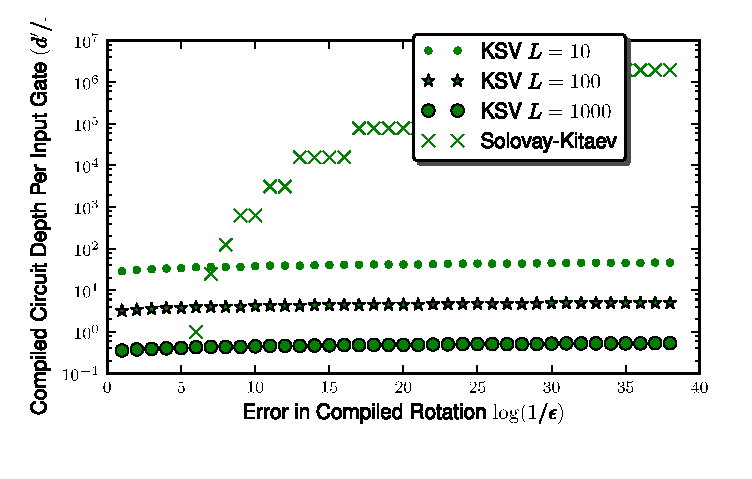
\includegraphics[width=3in]{figures/ksv-depth.eps}
\caption{Compiled circuit depth}
\label{fig:depth}
\end{figure}
\end{center}

\begin{center}
\begin{figure}[h!]
\label{fig:size}
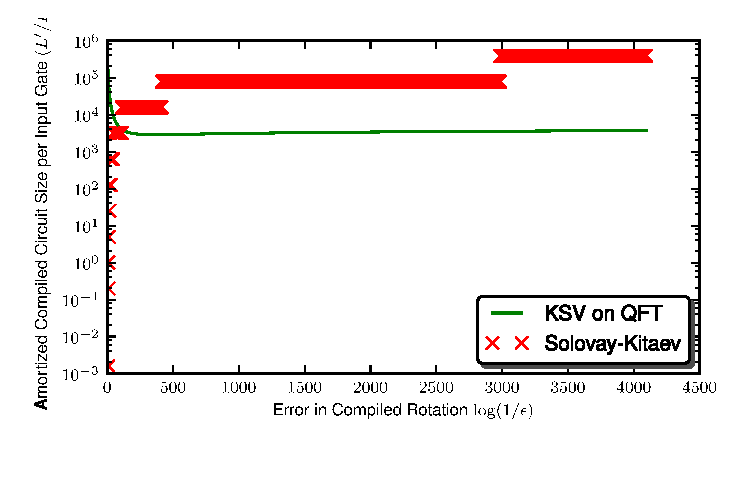
\includegraphics[width=3in]{figures/ksv-size.eps}
\caption{Compiled circuit size}
\label{fig:size}
\end{figure}
\end{center}

The discrete steps in SK's circuit size and depth are due
to the levels of recursion, which are conservatively chosen to meet
the desired precision. The initial step reflects the fact that even
before successive approximation, our initial generated sequences
(basic approximations in Section \ref{sec:sk-algo}) already meet large
desired precisions. As expected, KSV's depth compares very
favorably with Solovay-Kitaev.
The graphs are roughly linear in a log-log plot, with a non-linearity
for low precisions due to irregularities in the adder circuits for small
$n$.

Furthermore, we 

%%%%%%%%%%%%%%%%%%%%%%%%%%%%%%%%%%%%%%%%%%%%%%%%%%%%%%%%%%%%%%%%%%%%%%%%%%%%%%%
\subsection{Circuit Width and Classical Storage}
\label{subsec:results-width}

For the storage requirements, there is no direct comparison possible.
SK has a substantial classical storage requirement
at compile-time which is the dominant resource and is exponential with
the dimension $d$ of a quantum system of $d=2^n$ qubits.
The classical preprocessing time is
also intractable, but for most modern digital computers, storage space is the
bottleneck which is reached first, as shown in Figure \ref{fig:sk-space}.
SK uses no ancillae, so its circuit width overhead $W/W'$ would simply be
a constant 1.

%%%%%%%%%%%%%%%%%%%%%%%%%%%%%%%%%%%%%%%%%%%%%%%%%%%%%%%%%%%%%%%%%%%%%%%%%%%%%%%
%%%%%%%%%%%%%%%%%%%%%%%%%%%%%%%%%%%%%%%%%%%%%%%%%%%%%%%%%%%%%%%%%%%%%%%%%%%%%%%
% Make graph for sk-space.eps here using data on school macbook

%\begin{center}
%\begin{figure}[h!]
%\label{fig:sk-space}
%\includegraphics[width=3in]{sk-space.eps}
%\caption{SK classical preprocessing storage}
%\end{figure}
%\end{center}

On the other hand, KSV has no classical preprocessing stage, and its classical
storage needed for the side-processing in parallelized phase estimation is
efficient (linear in $n$). However, its circuit width overhead is

%%%%%%%%%%%%%%%%%%%%%%%%%%%%%%%%%%%%%%%%%%%%%%%%%%%%%%%%%%%%%%%%%%%%%%%%%%%%%%%
%%%%%%%%%%%%%%%%%%%%%%%%%%%%%%%%%%%%%%%%%%%%%%%%%%%%%%%%%%%%%%%%%%%%%%%%%%%%%%%
% Need a closed formula for circuit width overhead here, and in the table of
% asymptotic bounds in quals-report-definitions


%%%%%%%%%%%%%%%%%%%%%%%%%%%%%%%%%%%%%%%%%%%%%%%%%%%%%%%%%%%%%%%%%%%%%%%%%%%%%%%
%%%%%%%%%%%%%%%%%%%%%%%%%%%%%%%%%%%%%%%%%%%%%%%%%%%%%%%%%%%%%%%%%%%%%%%%%%%%%%%
% Find a way to make this two column to save vertical space!
% Find a way to make this accept PDF rather than EPS



\begin{center}
\begin{figure}[h!]
\label{fig:many-depth}
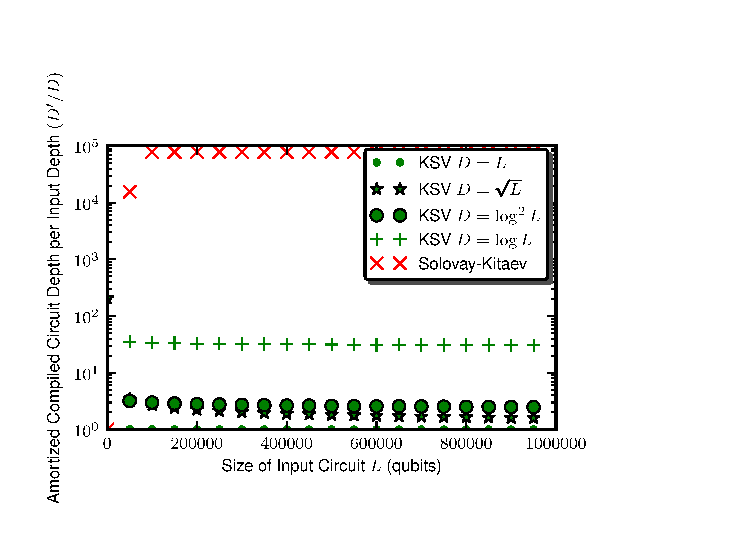
\includegraphics[width=3in]{figures/ksv-many-depths.eps}
\caption{Compiled circuit for various depth/size relationships}
\end{figure}
\end{center}

\begin{center}
\begin{figure}[h!]
\label{fig:one-size}
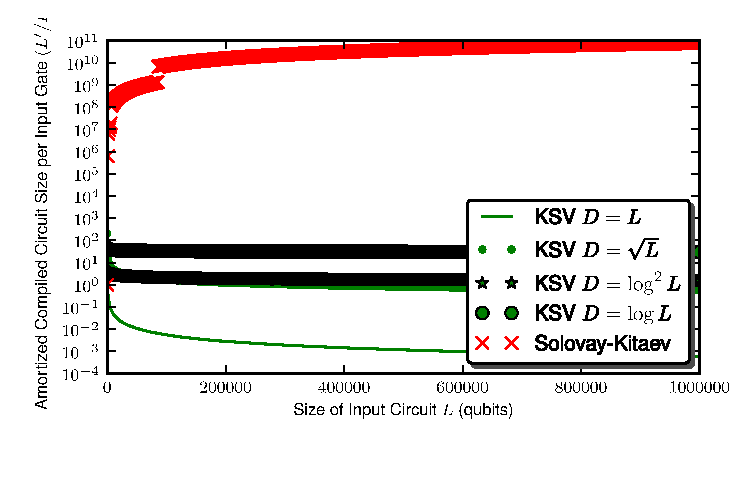
\includegraphics[width=3in]{figures/ksv-one-size.eps}
\caption{Compiled circuit per QFT size}
\end{figure}
\end{center}

The tradeoff between Solovay-Kitaev and Super-Kitaev can most clearly
be seen in the use of space. Solovay-Kitaev uses no ancillae at run-time,
but requires a classical preprocessing step to generate basic
approximations (precompiled sequences from the universal set). Although
we did not generate sequences beyond $l_0 = 9$ for $SU(4)$, the curve
indicates it would soon require terabytes of storage, even if a more
efficient encoding were used (e.g. programming in C instead of Python).
Super-Kitaev, on the other hand, requires no preprocessing space, but
has a (currently intractable) requirement for ancilla qubits are run-time
which tracks the circuit size as $O(n^2 \log n)$.

%%%%%%%%%%%%%%%%%%%%%%%%%%%%%%%%%%%%%%%%%%%%%%%%%%%%%%%%%%%%%%%%%%%%%%%%%%%%%%%
%%%%%%%%%%%%%%%%%%%%%%%%%%%%%%%%%%%%%%%%%%%%%%%%%%%%%%%%%%%%%%%%%%%%%%%%%%%%%%%
% Include graphs here for KSV ancillae usage and SK classical storage


\section{Conclusion and Future Directions}

In summary, we have seen the expected asymptotic bounds of both the
Solovay-Kitaev and Super-Kitaev quantum compiling algorithms reflected in
numerical resource comparisons. Solovay-Kitaev requires a large classical
preprocessing overhead but produces a more tractable number of compiled
gates and zero ancillae, albeit at larger circuit depth. This seems to be
a more reasonable choice for early experiments in running algorithms on an
80-qubit ion-trap quantum computer, where physical trapping constraints
make large numbers of qubits problematic but we are potentially willing to
wait a long time for the computation to complete. On the other hand, the
situation may change in the future when
quantum computers become more mature, scalable, and parallel;
when we become more ambitious in our
algorithm input sizes; and when the performance bottleneck becomes circuit depth.
In that case, Super-Kitaev may be preferrable.
Quantum computer engineers of the future will be able to use this work to
choose the most suitable quantum compiling technique currently available
as well as compare it to future compiling algorithms.

Moreover, the development of a compiler is intertwined with the
development of the underlying architecture. Just as classical programming
languages hint at what features would be desirable to move out of software
(and compile-time)
and into hardware (and run-time), Super-Kitaev provides some suggestions
to future quantum architectures. Hardware which seeks to take advantage of
this low-depth compiling would need to have a
"phase factory" for enacting the $\Lambda(e^{i\phi})$ gate, which would
included an efficient parallelized phase estimation routine. These are
novel resources which are currently not being considered in related literature.

\section{Acknowledgements}

The author would like to gratefully acknowledge the help of
his advisors Dave Bacon and Mark Oskin,
as well as Aram Harrow for the introduction to
Super-Kitaev and related expertise.

\bibliography{ksv-compiler}
\bibliographystyle{tocplain}

\end{document}
